This chapter will focus specifically on control rod cusping effects, which are the focus of this work.  First, a more thorough definition of the problem and motivation for solving it will be presented.  The next section will then present some of the solutions that have been used to minimize the cusping effects in the past, including a simplified decusping model implemented in MPACT itself.  The third section will then discuss some newer methods based on the sublpane CMFD scheme that have recently been implemented in MPACT.  Finally, a new ``sub-ray'' MOC method will be proposed to deal with the cause of the cusping effects on a more fundamental level.

\section{Background}

In Section \todo{section num}, some potential sources of errors for the 2D/1D scheme were introduced.  One of these was the error introduced by axial homogenization within a 2D MOC plane.  In some cases, this can be done without introducing significant errors.  For example, MPACT often homogenizes components outside the active fuel region, such as the end plugs and gaps at the end of the fuel rods.  However, when strong neutron absorbers, such as control rods, are homogenized axially in active fuel region, this has the effect of introducing absorption in regions where there should be none.  This effect is known as ``cusping,'' and is illustrated in Figure 

\begin{figure}
    \centering
    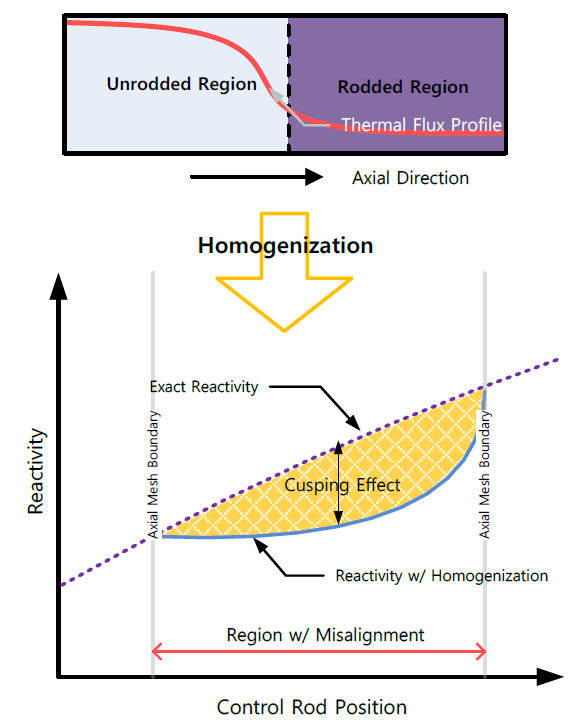
\includegraphics[width=0.4\textwidth]{figs/cusping_effect_Joo.png}
    \caption{Illustration of Rod ``Cusping''}\label{f:cuspingEffectJoo}
\end{figure}
\todo{cite}

In some cases, this is easily handled by setting up an appropriate axial mesh which prevents the need for the homogenization, but this is not always a practical solution.  Throughout the course of an entire cycle of operation (usually about 18 months), several different control banks in the reactor may move to a variety of positions to maintain criticality in the core.  Control rods in a PWR typically have step sizes of approximately 1.5 cm, but a typical MOC plane in MPACT is about 8 cm thick in the active fuel region.  In order to prevent cusping effects for an entire cycle, the user may have to create a very detailed axial mesh to ensure that all the control rod positions used throughout the cycle align with the edge of an MOC plane.  Not only is this tedious for the user, but it also greatly increases the computational burden due to the increased number of MOC planes.  Figure \ref{f:p4cuspingEffects} shows the calculated k-eff as a function of control rod position.  The cusping effects in this figure are further complicated by a heterogeneous rod with AIC and B$_4$C poison regions and a stainless steal tip.  Thus, cusping effects occur not just at the control rod tip, but also at material interfaces throughout the rod.

\begin{figure}
    \centering
    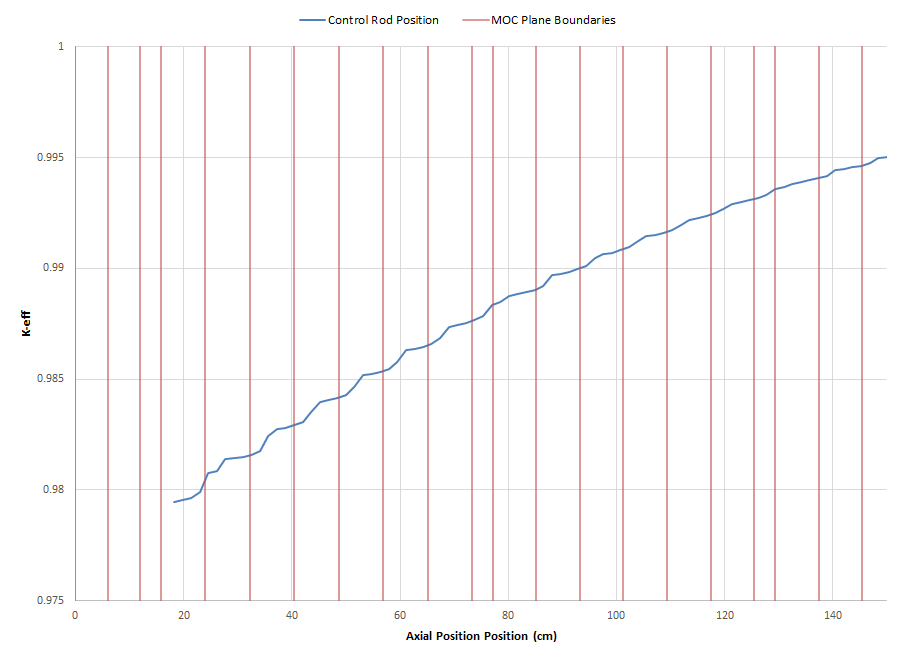
\includegraphics[width=0.8\textwidth]{figs/p4cuspingEffects.png}
    \caption{Control Rod Cusping Effects for 3x3 Assembly}\label{f:p4cuspingEffects}
\end{figure}

\section{Traditional Solutions}

\subsection{Nodal Codes}

\hl{Discuss ways people have addressed this in the past}

\subsection{2D/1D Codes}

Several codes that have employed the 2D/1D method in recent years have also required rod decusping methods.  MPACT currently uses a simple polynomial correction to the volume fractions used to homogenize the control rod\todo{cite Brendan m\& C 2015}.  To develop this method, a 3x3 assembly was set up with a control rod in the center assembly.  This problem was simulated with the rod tip at nine different positions in the plane.  These simulations were then repeated, but with the axial mesh refined so the rod tip aligned with a plane boundary.  The k-eff differences between the two sets of simulations were fitted with a sixth-order polynomial which is used in MPACT to reduce the volume fraction of the control rod by an appropriate amount to offset the cusping effects.  This process was repeated for different control rod materials such as AIC, B$_4$C, and Tungsten, since each material has unique cross-sections.  This method has the advantages of being simple to implement and requiring no increase in computational requirements.  However, the results obtained from this decusping method are tied to the control rod material and reactor model used to develop the corrections, limiting its usefulness to a small subset of reactors.

Another 2D/1D code is nTRACER, which is under active development by \hl{some people in Korea}.  To address rod cusping effects in nTRACER, \hl{Korean guy}, et al. developed a more general method than the polynomial correction method used by MPACT\todo{cite ICAPPS}.  This method pre-generates correction factors at the start of a simulation, rather than relying on hard-coded corrections.  To do this, the assembly that will have a partially inserted control rod is identified, and a single-plane 3x3 assembly problem is set up using the partially-rodded assembly and its neighbors.  The radial and axial cusping effects are then determined separately.  First, the radial cusping effects are determined by performing 2D MOC calculations on the 3x3 sub-domain with the rod fully inserted and fully withdrawn.  This provides radial flux profiles in the rodded assembly for both rodded and unrodded regions, as well as current coupling coefficients for CMFD for the rodded and unrodded CMFD nodes.  Once this is done, the rod is simulated at positions of 25\%, 50\%, and 75\% withdrawn from the plane.  To reduce runtime, these calculations are done using only 3D sub-plane CMFD.  This generates axial flux profiles for the full MOC plane for each of the possible rod positions.  During the full-core 2D/1D calculation, these axial flux profiles are then used to generate improved homogenized cross-sections for the MOC calculation using equation \ref{e:nTRACERdecusping}.

\begin{equation}\label{e:nTRACERdecusping}
\overline{\Sigma_i} = \frac{\phi_{rad,i}^R \phi_{ax,i}^R \Sigma_i^R h^R + \phi_{rad,i}^U \phi_{ax,i}^U \Sigma_i^U h^U}{\phi_{rad,i}^R \phi_{ax,i}^R h^R + \phi_{rad,i}^U \phi_{ax,i}^U h^U}
\end{equation}

\hl{DeCART?  Other 2D/1D codes?}

\section{Improved Decusping Methods}
\todo{Better Title?  Not that much ``better''}

This section discusses two new decusping treatments added to MPACT.  These methods rely on the sub-plane scheme described in section \todo{ref}.  The first method only treats the axial cusping effects, while the second method extends the first by also treating the radial decusping effects.

\subsection{Subplane Decusping}

\todo{Does this really belong anywhere?}

\begin{table}
\caption{Comparison of MPACT and DeCART subplane scheme results for C5G7-like rodded problem}
\begin{center}
\begin{tabular}{|l|c|c|c|c|c|c|}\hline
Plane & \multicolumn{2}{|c|}{k-eff Diff.} & \multicolumn{2}{|c|}{Max Power Diff.} & \multicolumn{2}{|c|}{Relative Runtime} \\ \cline{2-7}
Division & MPACT & DeCART & MPACT & DeCART & MPACT & DeCART \\ \hline
2 & 0.6 & 5.2 & 0.003\% & 0.04\% & 0.579 & 0.513 \\ \hline
3 & 1.9 & 7.7 & 0.004\% & 0.10\% & 0.408 & 0.327 \\ \hline
5 & 2.2 & 9.5 & 0.008\% & 0.11\% & 0.350 & 0.214 \\ \hline
10 & 1.2 & 9.8 & 0.020\% & 0.22\% & 0.253 & 0.058 \\ \hline
\end{tabular}
\end{center}
\end{table}

\begin{table}
\caption{Comparison of subplane scheme to traditional 2D/1D for VERA Progression Problem 4}
\begin{center}
\resizebox{\textwidth}{!}{\begin{tabular}{|l|c|c|c|c|c|c|c|c|}\hline
Number & k-eff Diff. & \multicolumn{2}{|c|}{Power Diff.} & \multicolumn{2}{|c|}{Outer Iterations} & \multicolumn{3}{|c|}{Runtime (core-hours)} \\\hline
of Planes & (pcm) & RMS & Max & Traditional & Subplane & Traditional & Subplane & Ratio ($\frac{Subplane}{Traditional}$) \\\cline{3-9}
32 & 0.01 & 0.001\% & 0.004\% & 29 & 30 & 21.0 & 16.2 & 0.77 \\\hline
46 & 0.01 & 0.018\% & 0.053\% & 14 & 21 & 10.3 & 8.9 & 0.86 \\\hline
62 & 0.04 & 0.023\% & 0.056\% & 12 & 20 & 12.4 & 11.5 & 0.93 \\\hline
77 & 0.04 & 0.022\% & 0.067\% & 12 & 21 & 13.0 & 11.4 & 0.88 \\\hline
\end{tabular}}
\end{center}
\end{table}

\begin{table}
\caption{Comparison of subplane scheme to traditional 2D/1D for VERA Progression Problem 5}
\begin{center}
\resizebox{\textwidth}{!}{\begin{tabular}{|l|c|c|c|c|c|c|c|c|}\hline
Number & k-eff Diff. & \multicolumn{2}{|c|}{Power Diff.} & \multicolumn{2}{|c|}{Outer Iterations} & \multicolumn{3}{|c|}{Runtime (core-hours)} \\\hline
of Planes & (pcm) & RMS & Max & Traditional & Subplane & Traditional & Subplane & Ratio ($\frac{Subplane}{Traditional}$) \\\cline{3-9}
32 & 0.01 & 0.004\% & 0.008\% & 28 & 29 & 996  & 1325 & 1.33 \\\hline
46 & 0.11 & 0.044\% & 0.111\% & 13 & 29 & 691  & 829  & 1.20 \\\hline
62 & 0.07 & 0.028\% & 0.190\% & 12 & 46 & 880  & 918  & 1.04 \\\hline
77 & 0.08 & 0.030\% & 0.184\% & 12 & 45 & 1090 & 1013 & 0.93 \\\hline
\end{tabular}}
\end{center}
\end{table}

\subsection{Auxiliary 1D Collision Probabilities}

The CMFD homogenized flux can be calculated as follows:

\begin{equation}\label{e:CMFDsubplaneFlux}
\phi^k_{g,c} = \frac{\sum_{i=1}^{N_{FSR}} \phi^{k=1}_{g,i} V_i}{\sum_{i=1}^{N_{FSR}} V_i} c_{g,c}
\end{equation}

The subscripts $i$, $g$, and $c$ are fine mesh cell indexes, energy group indexes, and CMFD cell indexes, respectively.  The factor $c_{g,c}$ is a group- and cell-dependent scaling factor for the subplane method.  This factor provides an axial shape to the MOC flux using the previous iterate.  It is defined as follows:

\begin{equation}\label{e:CMFDsubplaneFactor}
c_{g,c} = \frac{\phi^{k-1}_{g,c}}{\overline{\phi^k_{g,c}}}
\end{equation}

where the average flux in the denominator is defined by

\begin{equation}\label{e:CMFDaverageFlux}
\phi^k_{g,c} = \frac{\sum_{i=1}^{N_{FSR}} \phi^{k=1}_{g,i} V_i}{\sum_{i=1}^{N_{FSR}} V_i}
\end{equation}

This definition of the subplane factor provides axial shape while still preserving the volume-averaged flux and reaction rates in each pin cell in the MOC plane.

The CMFD homogenized cross-sections can be calculated using the MOC flux:

\begin{equation}\label{e:CMFDhomXS}
\Sigma_{x,c} = \frac{\sum_{i=1}^{N_{FSR}} \phi_{g,i}\Sigma_{x,g,i}V_i}{\sum_{i=1}^{N_{FSR}} \phi_{g,i}V_i}
\end{equation}

Multiplying equations \ref{e:CMFDsubplaneFlux} and \ref{e:CMFDhomXS} gives the reaction rate in the pin cell.

When using the embedded solver, a radial flux profile is obtained from the solver.  The process described above is followed for the nodes around the partially inserted rod.  However, instead of the MOC flux, the radial flux from the embedded solver is used.  This allows subplanes with partially inserted control rods to have different cross-sections based on the radial flux profile around the tip of the control rod.

\hl{The flux coming out of the embedded solver is treated as a shape function and scaled to preserve the MOC flux.}

\hl{Need to make sure reaction rates are preserved I think}.

\hl{A constant current is used for all subplanes.  This does not provide the most accurate solution, but ensures stability and neutron balance.}

\hl{When projecting, the subplane fluxes scale MOC fluxes.  Reference equation.}

\hl{The cross-sections can be modified by mixing the rodded and unrodded cross-sections.  Equation from Han Joo cusping paper.}

\section{Future Work}

\subsection{Auxiliary Solver}

\hl{Something better than 1D CPM... Namely MOC}

\subsection{Radial Transverse Leakage Source}

\hl{sub-plane dependent dhats/currents}

\subsection{Axial Transverse Leakage Source}

\hl{Spatially dependent axial TL}

\subsection{Sub-Ray MOC}

\hl{Boom}